\chapter{Background}
\label{ch:background}

This chapter introduces the three building blocks needed to understand \NS:
the Transformer with its KV cache, state-space models (Mamba and Mamba-2), and
Mixture-of-Experts layers.

\section{The Transformer and the KV Cache}

\subsection{Self-Attention}

A Transformer layer consists of a self-attention block followed by a
feed-forward network (FFN)~\cite{vaswani2017attention}. Given a sequence of $n$
token representations stacked as the rows of $X \in \mathbb{R}^{n \times d}$,
self-attention forms queries, keys and values by linear projection,
$Q = XW_Q$, $K = XW_K$, $V = XW_V$, and computes
\begin{equation}
  \operatorname{Attention}(Q,K,V) =
  \operatorname{softmax}\!\left(\frac{QK^{\top}}{\sqrt{d_k}}\right)V ,
  \label{eq:attention}
\end{equation}
where $d_k$ is the dimension of each key. The matrix $QK^{\top}$ has $n \times
n$ entries, one for every pair of tokens. This is what gives attention its
power---any token can retrieve information from any other token in a single
step---and also what makes it expensive: both the time and the memory of this
product grow as $O(n^2)$. Doubling the input length quadruples the work in
every attention layer. Figure~\ref{fig:complexity} contrasts this growth with
the linear growth of a state-space layer.

\begin{figure}[htbp]
  \centering
  % Attention O(n^2) vs Mamba O(n): relative per-layer cost against sequence length
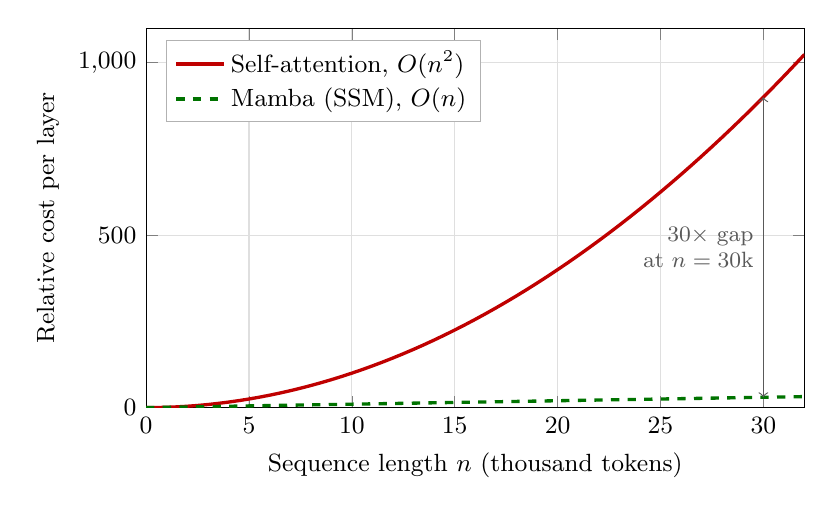
\begin{tikzpicture}
\begin{axis}[
  width=0.82\linewidth, height=6.4cm,
  xlabel={Sequence length $n$ (thousand tokens)},
  ylabel={Relative cost per layer},
  xmin=0, xmax=32, ymin=0, ymax=1100,
  domain=0:32, samples=65,
  grid=major, grid style={gray!25},
  legend pos=north west, legend cell align=left,
  legend style={font=\small, draw=gray!60},
  tick label style={font=\small}, label style={font=\small}]
\addplot[very thick, red!75!black] {x^2};
\addlegendentry{Self-attention, $O(n^2)$}
\addplot[very thick, green!45!black, dashed] {x};
\addlegendentry{Mamba (SSM), $O(n)$}
\draw[<->, gray!70!black] (axis cs:30,30) -- (axis cs:30,900)
  node[midway, left, font=\footnotesize, align=right] {$30\times$ gap\\at $n=30$k};
\end{axis}
\end{tikzpicture}

  \caption[Quadratic cost of self-attention versus linear cost of Mamba]{Relative
  per-layer cost of self-attention, $O(n^2)$, and of a Mamba layer, $O(n)$, as
  the sequence grows (both normalised to 1 at $n=1$k tokens; drawn by the
  author).}
  \label{fig:complexity}
\end{figure}

\subsection{Autoregressive Generation and the KV Cache}

Language models generate text one token at a time. To produce token $t+1$ the
newest token must attend to all $t$ tokens before it. Recomputing the keys and
values of those earlier tokens at every step would be wasteful, so
implementations store them in a \emph{KV cache} and append one new key--value
pair per layer for every generated token. The cache removes redundant
computation, but it introduces two costs that grow with the context:
\begin{itemize}
  \item \textbf{Memory.} The cache holds one entry per past token per attention
        layer, so its size grows linearly and without bound as the context
        lengthens.
  \item \textbf{Time per token.} Every new token must read the whole cache, so
        the cost of generating a token also grows linearly with the context,
        and the total cost of generating a sequence grows quadratically.
\end{itemize}
More cache means more GPU memory and more memory traffic per token, so fewer
requests fit on a GPU and each one runs more slowly. Figure~\ref{fig:kvcache}
illustrates the difference from a state-space layer, whose state does not grow.

\begin{figure}[htbp]
  \centering
  % KV cache growth vs constant-size SSM state during generation
\begin{tikzpicture}[font=\small]
\node[font=\small\bfseries, anchor=west] at (0,0.85) {Attention layer: KV cache};
\node[font=\small\bfseries, anchor=west] at (7.6,0.85) {Mamba layer: SSM state};
\foreach \n/\y/\lab in {4/0/{$t=4$}, 8/-0.95/{$t=8$}, 16/-1.9/{$t=16$}}{
  \node[anchor=east] at (-0.15,\y) {\lab};
  \foreach \i in {1,...,\n}{
    \draw[fill=red!22, draw=red!60!black] ({(\i-1)*0.4},{\y-0.2}) rectangle ++(0.34,0.4);
  }
  \draw[fill=green!25, draw=green!40!black] (7.6,{\y-0.2}) rectangle ++(1.6,0.4);
  \node[font=\footnotesize] at (8.4,\y) {$h_t$};
}
\draw[-{Stealth}, gray!70!black] (0,-2.55) -- (6.2,-2.55)
  node[midway, below, font=\footnotesize] {one $(k,v)$ entry per past token: memory $\propto t$};
\node[font=\footnotesize, anchor=north] at (8.4,-2.62) {fixed size: memory $\propto 1$};
\end{tikzpicture}

  \caption[KV cache growth versus a constant-size SSM state]{During generation
  an attention layer appends one key--value entry per token, whereas a Mamba
  layer overwrites a state of fixed size (drawn by the author).}
  \label{fig:kvcache}
\end{figure}

Techniques such as Grouped-Query Attention~\cite{ainslie2023gqa}, in which
many query heads share a small number of key--value heads, reduce the size of
each cache entry but not the way the cache scales. For very long-context tasks
a pure Transformer therefore remains expensive and inefficient.

\section{State-Space Models}

\subsection{From Continuous Systems to Sequence Layers}

A state-space model describes a system through a hidden state $h(t) \in
\mathbb{R}^{N}$ that evolves under an input signal $x(t)$ and produces an
output $y(t)$:
\begin{equation}
  h'(t) = A\,h(t) + B\,x(t), \qquad y(t) = C^{\top} h(t).
  \label{eq:ssm-cont}
\end{equation}
To apply this to a sequence of tokens, the system is discretised with a step
size $\Delta$. Under the commonly used zero-order hold rule the discrete
parameters are $\bar{A} = \exp(\Delta A)$ and
$\bar{B} = (\Delta A)^{-1}\bigl(\exp(\Delta A) - I\bigr)\,\Delta B$, which
gives the recurrence~\cite{gu2021s4,gu2023mamba}
\begin{equation}
  h_t = \bar{A}\,h_{t-1} + \bar{B}\,x_t, \qquad y_t = C^{\top} h_t .
  \label{eq:ssm-disc}
\end{equation}
In words, the model reads the text one token at a time and keeps one small
``note'' in memory, the state $h_t$. After each token it updates the note,
writing in what matters and letting the rest decay. The note has the same size
whether the text is one thousand or one million tokens long.
Figure~\ref{fig:ssm} shows this recurrence unrolled over three steps.

\begin{figure}[htbp]
  \centering
  % Unrolled state-space recurrence  h_t = A_t h_{t-1} + B_t x_t,  y_t = C_t^T h_t
\begin{tikzpicture}[
  font=\small, >={Stealth},
  state/.style={circle, draw=green!40!black, fill=green!18, minimum size=1.05cm, inner sep=0pt},
  io/.style={rectangle, rounded corners=2pt, draw=gray!70, fill=gray!10, minimum width=0.9cm, minimum height=0.6cm}]
\node[state] (h0) at (0,0)   {$h_{t-1}$};
\node[state] (h1) at (3.4,0) {$h_{t}$};
\node[state] (h2) at (6.8,0) {$h_{t+1}$};
\node (l) at (-2.0,0) {$\cdots$};
\node (r) at (8.8,0)  {$\cdots$};
\foreach \k/\x/\lab in {0/0/{t-1}, 1/3.4/{t}, 2/6.8/{t+1}}{
  \node[io] (x\k) at (\x,-1.9) {$x_{\lab}$};
  \node[io] (y\k) at (\x,1.9)  {$y_{\lab}$};
  \draw[->] (x\k) -- node[right, font=\footnotesize] {$B_{\lab}$} (h\k);
  \draw[->] (h\k) -- node[right, font=\footnotesize] {$C_{\lab}$} (y\k);
}
\draw[->] (l) -- (h0);
\draw[->] (h0) -- node[above, font=\footnotesize] {$A_{t}$} (h1);
\draw[->] (h1) -- node[above, font=\footnotesize] {$A_{t+1}$} (h2);
\draw[->] (h2) -- (r);
\end{tikzpicture}

  \caption[Unrolled state-space recurrence]{The state-space recurrence unrolled
  over time: each state $h_t$ depends only on the previous state and the
  current input (drawn by the author).}
  \label{fig:ssm}
\end{figure}

Because the update in Eq.~\eqref{eq:ssm-disc} touches only $h_{t-1}$ and $x_t$,
processing $n$ tokens costs $O(n)$ time, and generating a new token costs the
same amount of work and memory no matter how long the context already is.

\subsection{Mamba: Selective State Spaces}

In early SSMs such as S4~\cite{gu2021s4} the matrices $A$, $B$ and $C$ are
fixed after training, so every token is written into the state in the same
way. Text is not like that: some tokens are essential and many are filler.
Mamba~\cite{gu2023mamba} makes the parameters depend on the current input,
\begin{equation}
  h_t = \bar{A}(x_t)\,h_{t-1} + \bar{B}(x_t)\,x_t, \qquad
  y_t = C(x_t)^{\top} h_t ,
  \label{eq:mamba}
\end{equation}
so that the model can \emph{select} what to remember. When $\bar{A}(x_t)$ is
close to the identity and $\bar{B}(x_t)$ is small, the token is effectively
ignored and the state is carried forward unchanged; in the opposite case the
state is reset and overwritten. The Mamba block wraps this selective SSM with a
linear projection, a short convolution and a gated branch
(Figure~\ref{fig:mamba-block}) and is stacked like a Transformer block, without
any attention.

\begin{figure}[htbp]
  \centering
  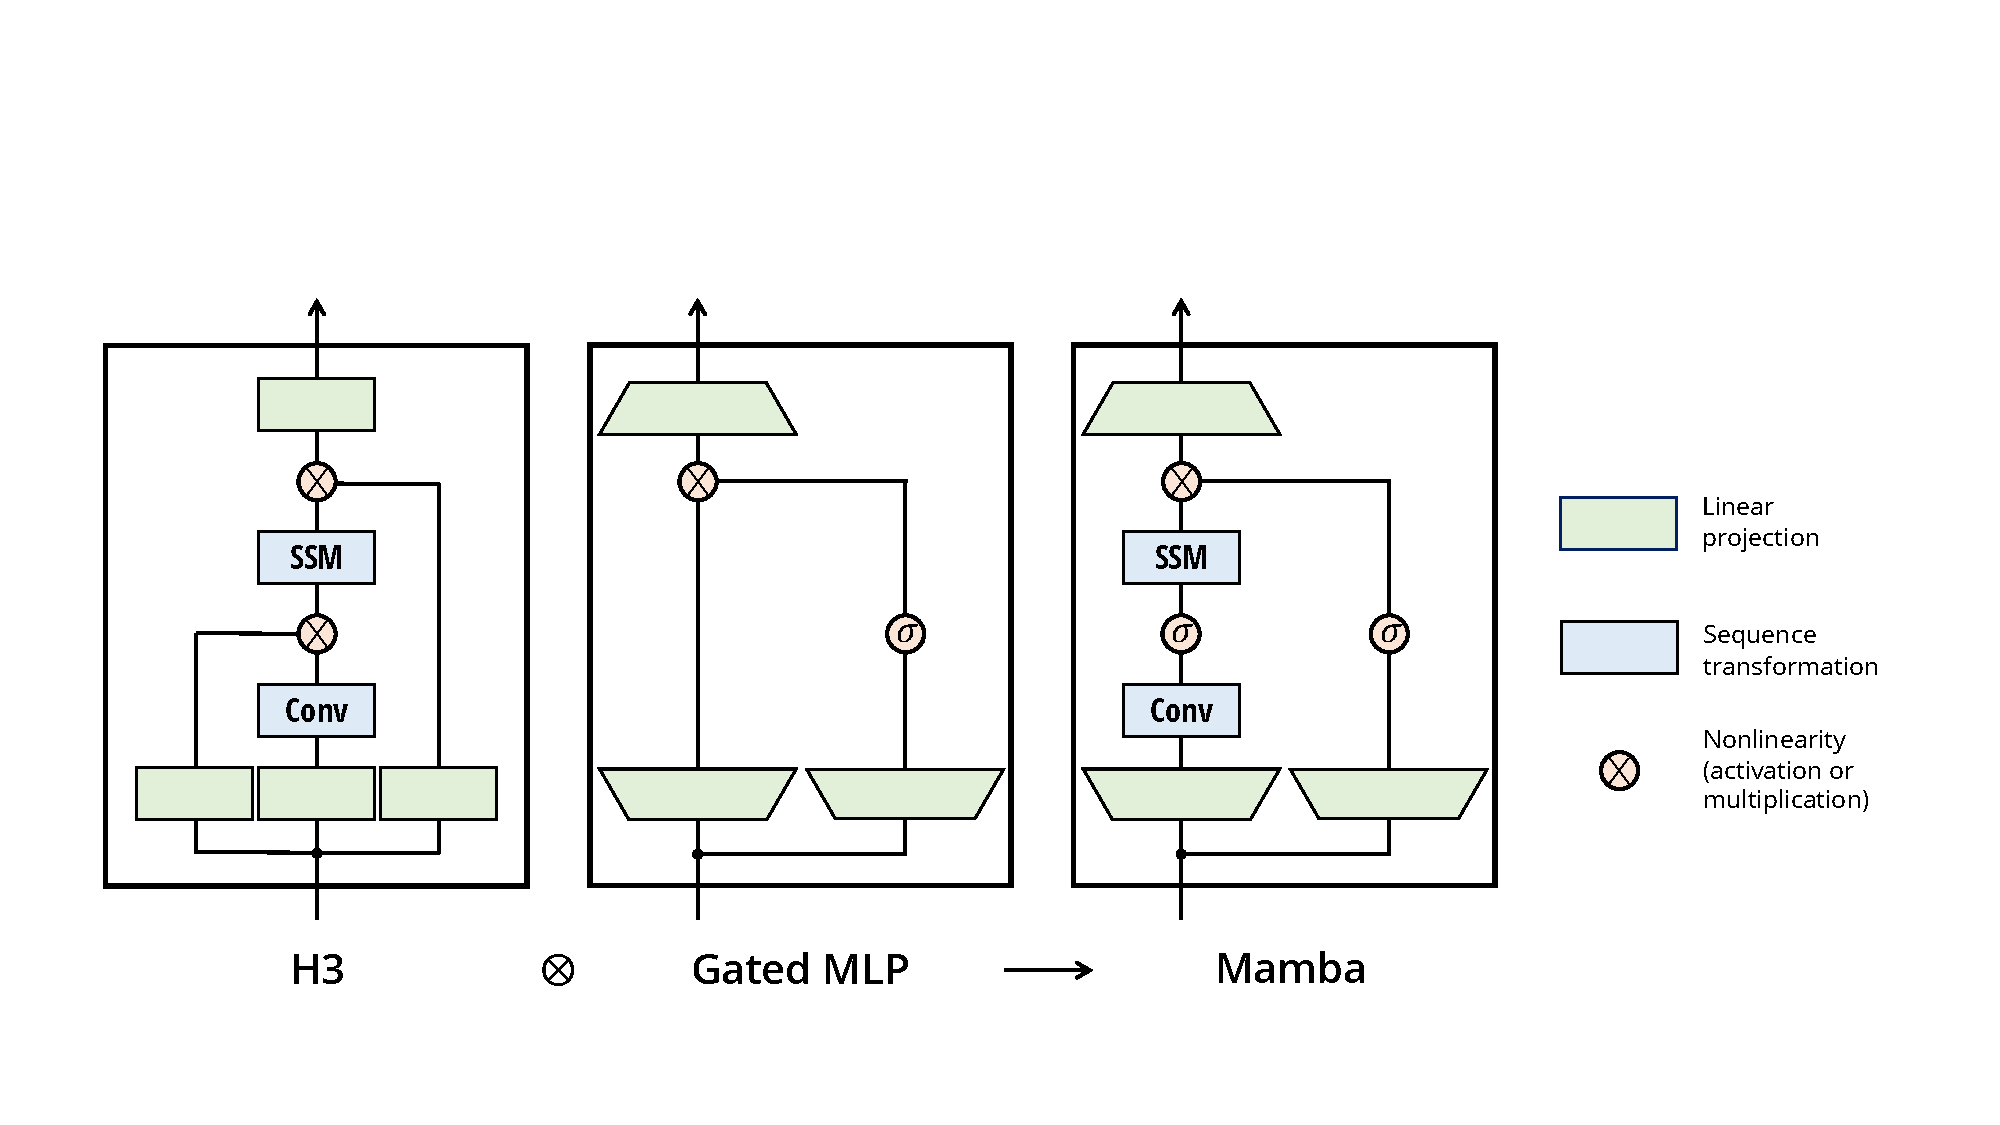
\includegraphics[width=0.9\linewidth]{mamba-fig03-block.pdf}
  \caption[The Mamba block compared with the H3 and gated-MLP blocks]{The Mamba
  block combines the H3 block, the basis of most earlier SSM architectures,
  with the gated MLP block. \source{Gu and Dao (2023)~\cite{gu2023mamba}, Fig.~3}}
  \label{fig:mamba-block}
\end{figure}

\subsection{Mamba-2 and State Space Duality}
\label{sec:mamba2}

Mamba-2~\cite{dao2024mamba2} starts from an observation about
Eq.~\eqref{eq:mamba}. Unrolling the recurrence shows that the whole layer is a
single matrix multiplication $y = Mx$, where
\begin{equation}
  M_{ji} = C_j^{\top} A_j A_{j-1} \cdots A_{i+1} B_i \quad (j \ge i),
  \label{eq:ssd}
\end{equation}
and $M_{ji}=0$ for $j<i$. Matrices of this form are called
\emph{semiseparable}. Dao and Gu show that a restricted form of masked
attention produces exactly the same family of matrices, which they call
\emph{structured state space duality} (SSD): the same sequence transformation
can be computed either as a linear-time recurrence (the SSM view) or as a
matrix product (the attention view).

Mamba-2 exploits both views. It restricts each $A_t$ to a scalar times the
identity and groups channels into \emph{heads}, much like attention heads.
During training, the sequence is cut into chunks; within a chunk the layer is
computed with ordinary matrix multiplications, which GPUs execute very
efficiently, and the states are passed between chunks with the recurrence. As
a result the SSD algorithm is 2--8$\times$ faster than Mamba's sequential scan
while keeping linear scaling in sequence length. During generation Mamba-2
falls back to the pure recurrence and so keeps a constant-size state. The block
is also simplified (Figure~\ref{fig:mamba2-block}), which makes it easier to
parallelise across GPUs.

\begin{figure}[htbp]
  \centering
  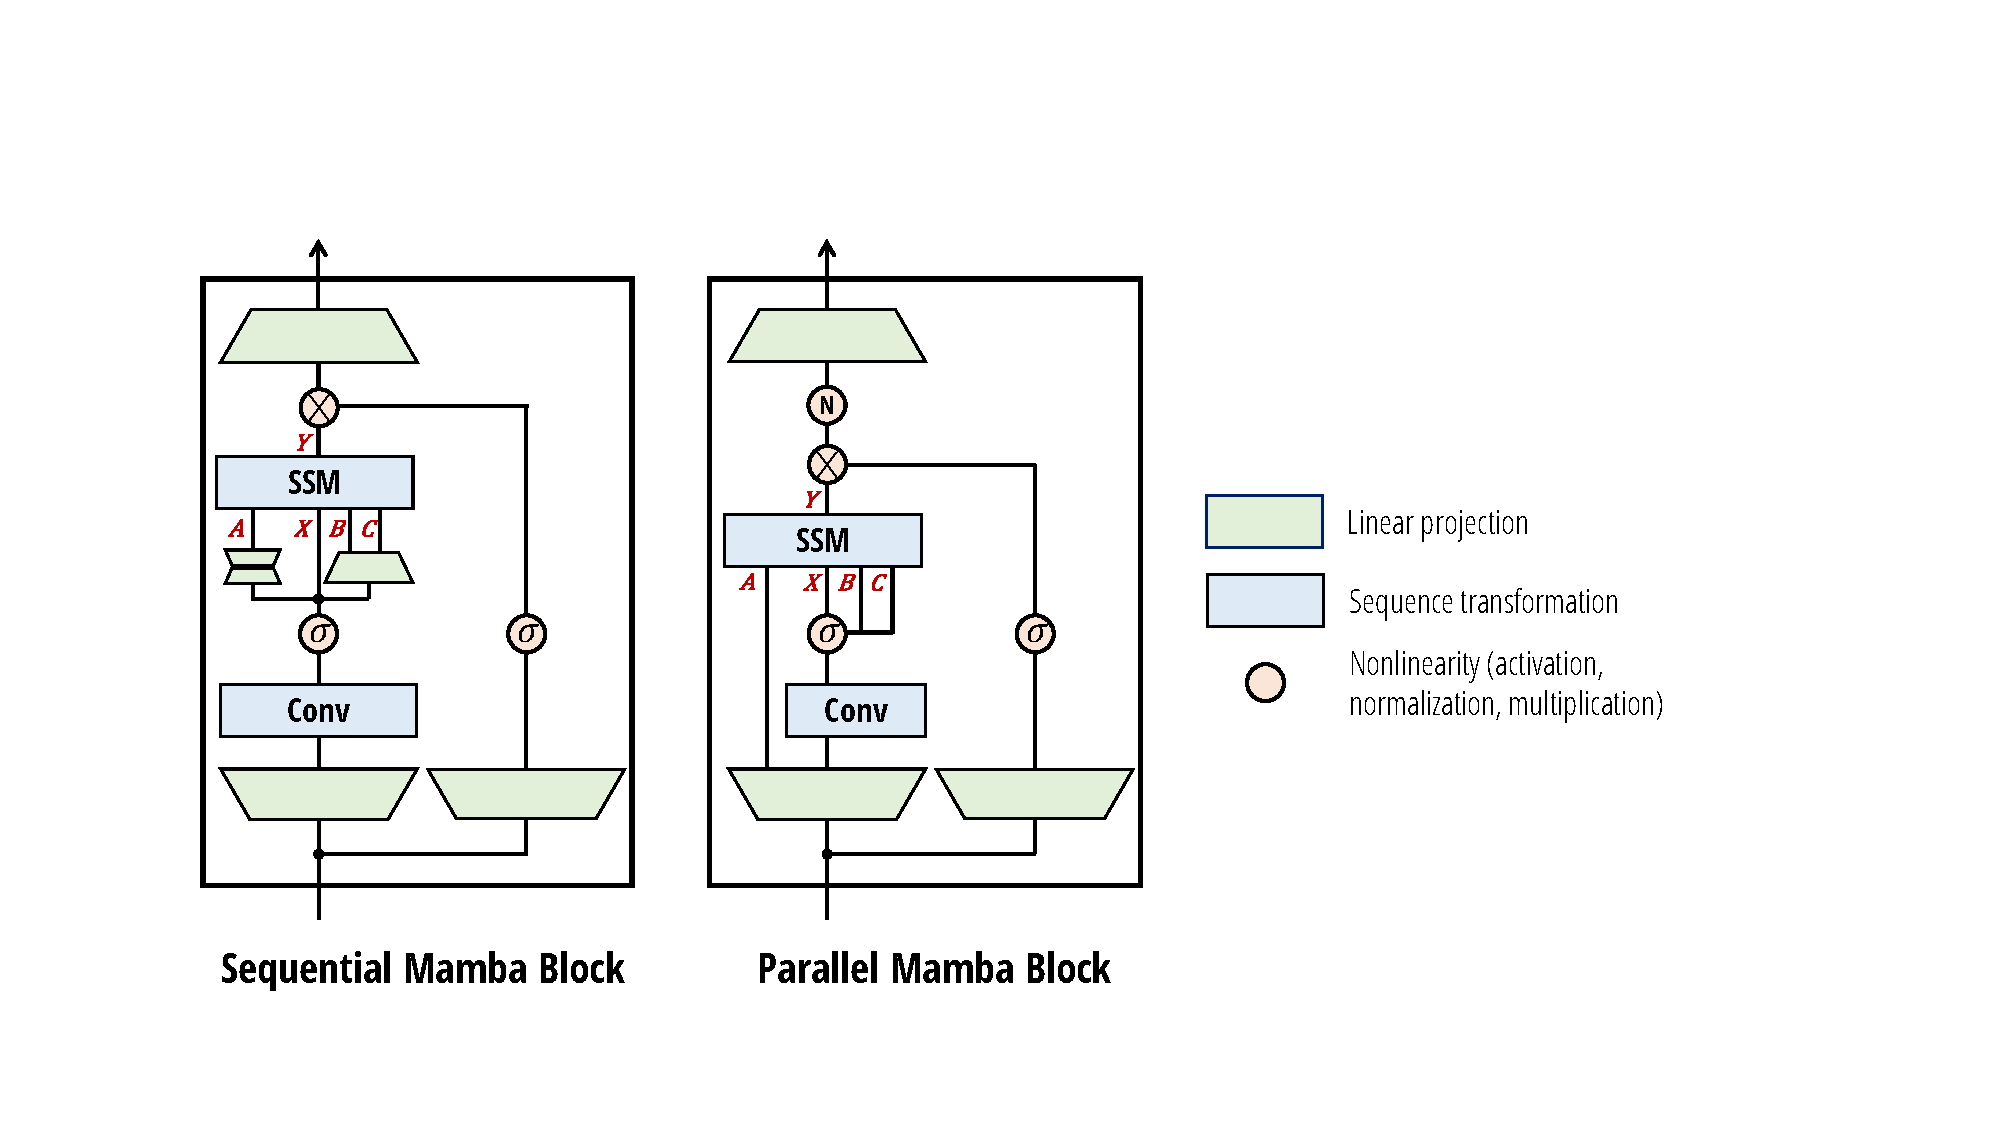
\includegraphics[width=0.78\linewidth]{mamba2-fig06-block.pdf}
  \caption[The Mamba-2 block]{The Mamba-2 block simplifies the Mamba block by
  removing sequential linear projections; the SSM parameters are produced in
  parallel at the start of the block. \source{Dao and Gu
  (2024)~\cite{dao2024mamba2}, Fig.~6}}
  \label{fig:mamba2-block}
\end{figure}

\subsection{What a State-Space Layer Cannot Do}

The strength of an SSM is also its weakness. Everything the layer knows about
the past must fit into a state of fixed size, so the state is necessarily a
lossy summary. Tasks that need an exact copy of something seen long ago---a
phone number from a long list, a variable name defined thousands of lines
earlier---are precisely where pure SSMs fall behind
Transformers~\cite{waleffe2024empirical}. Attention has the opposite profile:
perfect recall at high cost. Table~\ref{tab:attn-vs-ssm} summarises the
contrast, which is the motivation for hybrid models.

\begin{table}[htbp]
\centering
\small
\caption{Self-attention and Mamba-2 layers compared}
\label{tab:attn-vs-ssm}
\begin{tabularx}{\linewidth}{@{}P{4.2cm}LL@{}}
\toprule
\textbf{Property} & \textbf{Self-attention} & \textbf{Mamba-2 (SSM)} \\
\midrule
Compute for $n$ tokens & $O(n^2)$ & $O(n)$ \\
Memory during generation & KV cache, grows as $O(n)$ & Fixed-size state, $O(1)$ \\
Work per generated token & Grows with context & Constant \\
Access to past tokens & Exact, to every token & Compressed summary \\
Typical weakness & Cost on long contexts & Exact recall and copying \\
\bottomrule
\end{tabularx}
\end{table}

\section{Mixture-of-Experts}

\subsection{The Basic Idea}

In a standard Transformer, roughly two thirds of the parameters sit in the
feed-forward networks, and every token passes through all of them. A
Mixture-of-Experts layer~\cite{shazeer2017moe} replaces the single FFN with
$N$ smaller FFNs called \emph{experts}, $E_1,\dots,E_N$, together with a small
\emph{router} network. For each token $x$ the router produces a score for every
expert, only the $k$ highest-scoring experts are evaluated, and their outputs
are combined:
\begin{equation}
  y = \sum_{i \,\in\, \operatorname{TopK}(g(x),\,k)} g_i(x)\, E_i(x),
  \qquad E_i(x) = W^{(i)}_{2}\,\sigma\!\bigl(W^{(i)}_{1}x\bigr).
  \label{eq:moe}
\end{equation}
Here $g(x)$ is the vector of router scores and $\sigma$ is a non-linearity.
Figure~\ref{fig:moe} sketches the layer. The experts that are not selected do
no work for this token, so the \emph{total} parameter count grows with $N$
while the \emph{active} parameter count and the FLOPs per token grow only with
$k$. This is how a model can be very large and still cheap to run.

\begin{figure}[htbp]
  \centering
  % Mixture-of-Experts layer: router scores all experts, only the top-k run
\begin{tikzpicture}[
  font=\small, >={Stealth},
  box/.style={rectangle, rounded corners=3pt, draw=gray!70!black, minimum height=0.75cm},
  on/.style={box, fill=orange!35, minimum width=0.95cm},
  off/.style={box, fill=gray!12, text=gray!70, draw=gray!45, minimum width=0.95cm}]
\node[box, fill=blue!12, minimum width=1.5cm] (x) at (0,0) {token $x$};
\node[box, fill=blue!22, minimum width=1.9cm, align=center] (r) at (0,-1.6) {Router $g(x)$};
\node[off] (e1) at (-4.2,-3.6) {$E_1$};
\node[on]  (e2) at (-3.0,-3.6) {$E_2$};
\node[off] (e3) at (-1.8,-3.6) {$E_3$};
\node[off] (e4) at (-0.6,-3.6) {$E_4$};
\node[on]  (e5) at (0.6,-3.6)  {$E_5$};
\node[off] (e6) at (1.8,-3.6)  {$E_6$};
\node (dots) at (2.8,-3.6) {$\cdots$};
\node[on]  (en) at (3.9,-3.6)  {$E_N$};
\node[circle, draw=gray!70!black, fill=white, inner sep=1.5pt] (s) at (0,-5.4) {$\sum$};
\node[box, fill=blue!12, minimum width=1.5cm] (y) at (0,-6.7) {output $y$};
\draw[->] (x) -- (r);
\foreach \e/\w in {e2/g_2, e5/g_5, en/g_N}{
  \draw[->, thick, orange!70!black] (r.south) -- (\e.north);
  \draw[->, thick, orange!70!black] (\e.south) -- node[pos=0.45, fill=white, inner sep=1pt, font=\footnotesize] {$\w$} (s);
}
\foreach \e in {e1,e3,e4,e6}{ \draw[->, gray!45, densely dashed] (r.south) -- (\e.north); }
\draw[->] (s) -- (y);
\node[font=\footnotesize, align=left, anchor=west] at (4.7,-1.6) {scores all $N$ experts,\\keeps the top-$k$};
\node[font=\footnotesize, align=left, anchor=west] at (4.7,-3.6) {only $k$ experts run;\\the rest stay idle};
\end{tikzpicture}

  \caption[Mixture-of-Experts layer with router and top-$k$ selection]{A
  Mixture-of-Experts layer: the router scores all $N$ experts and only the
  top-$k$ (shaded) are executed and summed (drawn by the author).}
  \label{fig:moe}
\end{figure}

\subsection{Practical Issues}

Sparse routing introduces problems that dense models do not have.
\begin{itemize}
  \item \textbf{Load balancing.} If the router sends most tokens to a few
        favourite experts, the rest are wasted. GShard~\cite{lepikhin2020gshard}
        adds an auxiliary loss that encourages even usage, and
        DeepSeek-V3~\cite{deepseek2024v3} adjusts a per-expert bias instead so
        that no extra loss term is needed.
  \item \textbf{Memory.} Idle experts still occupy memory. All $N$ experts
        must be loaded even though only $k$ run for a given token.
  \item \textbf{Memory bandwidth and communication.} Each token may use a
        different set of experts, so the weights that must be read change from
        token to token, and in a multi-GPU deployment tokens must be shipped to
        whichever device holds their experts.
\end{itemize}
These hardware-level costs are the starting point for LatentMoE, the MoE
variant used in \NS, which is described in Chapter~\ref{ch:arch}.
